\begin{figure*}[t!]
\centering
    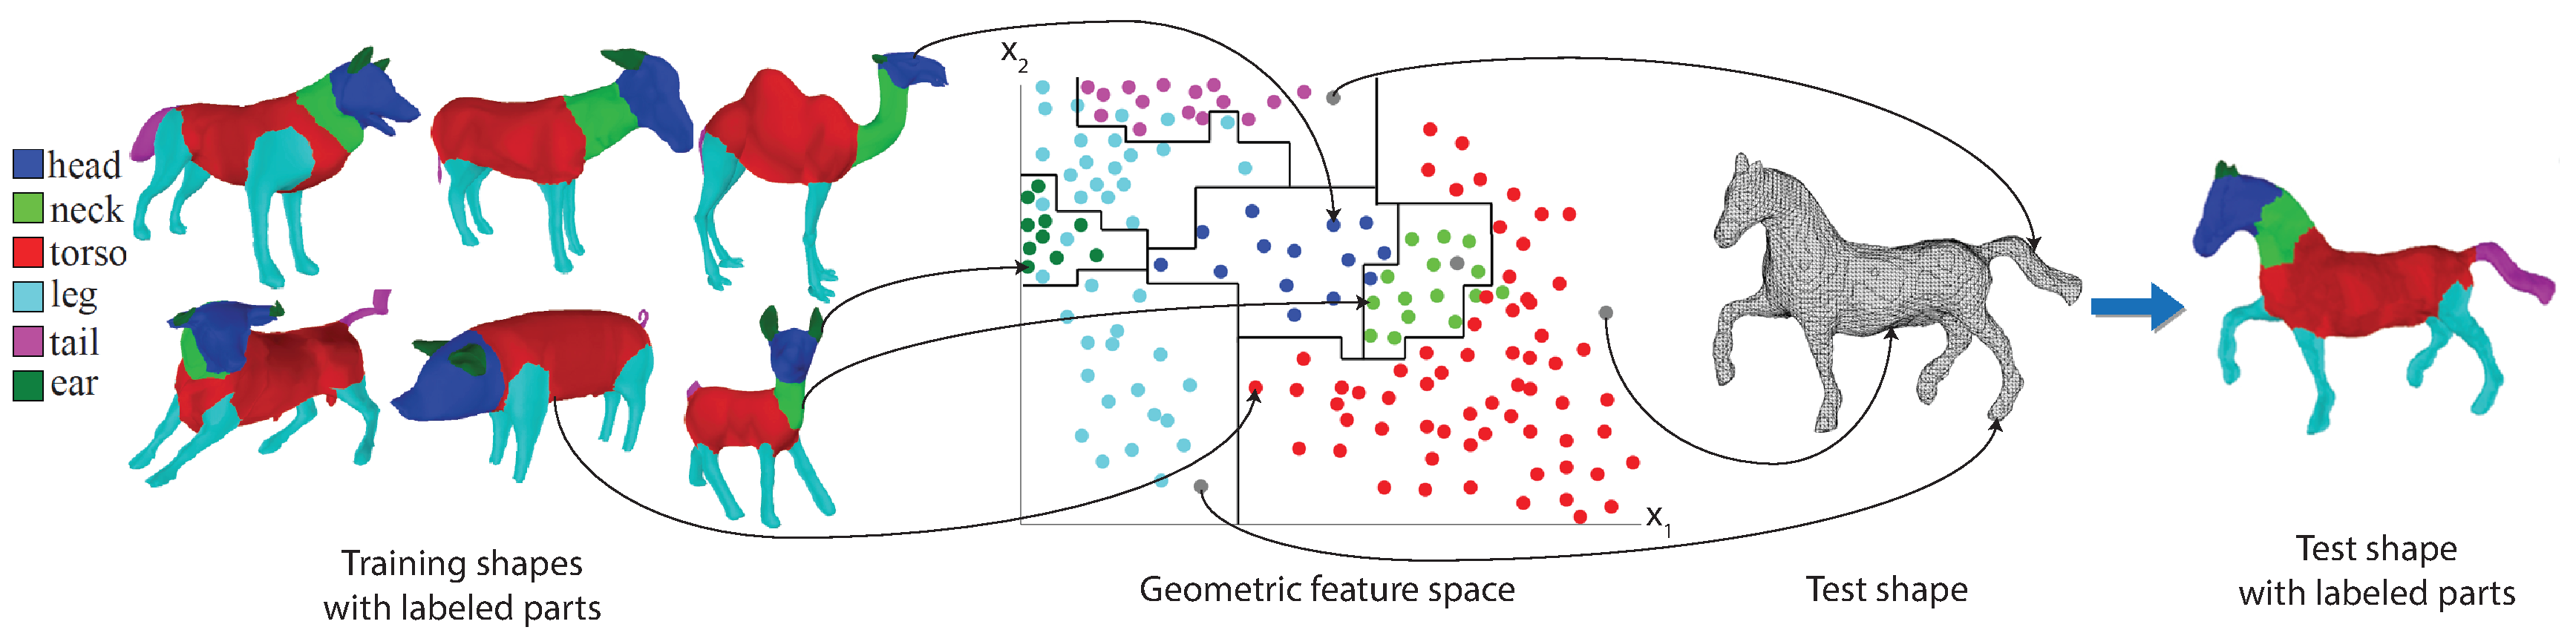
\includegraphics[width=1.0\textwidth]{fig/img/overview_seg.pdf}
    %\vspace{-.5cm}
    \caption{
Pipeline of a supervised segmentation algorithm \cite{Kalogerakis:2010:LMS}. Given a set of shapes with labeled parts, the points of each shape are embedded in a common feature space based on their local geometric descriptors (a color is assigned to points depending on their given part label). A classifier is learned to split the feature space into regions corresponding to each part label. Given a test shape, its points (shown in grey) are first embedded in the same space. Then part labels are inferred for all its points based on the learned classifier and an underlying structured probabilistic model (Section \ref{sec:segmentation}).
}
\label{fig:overview_seg}
\end{figure*}

